\chapter{Implemented Improvements to PlanetLab Server Manager}
\label{chapter:improve}
This Chapter will discuss improvements made to the PlanetLab application. The improvements are based on the analysis made in the Section~\ref{section:improvement}. The implementation details will be described and shown. The goal of the re-implementation is to make the \texttt{plmbng} tool simple to use, easier to contribute into by re-writing it fully into Python~3, using good coding practices, remove any post-installations steps and making small improvements. Improvements includes:
\begin{itemize}
	\item Removing result limitation by dynamically creating menu using Python \texttt{list}.
	\item Adding support to use application as library by logically separating each function.
	\item Increasing readability and improve orientation in the application by renaming menu components and using descriptive functions names.
	\item Eliminating pre and post installation steps by using automatic \texttt{pip} dependency installer.
	\item Improving credentials set up by adding internal text editor.
	\item Extending Windows support to several functions by detecting operating system and dynamically changing parameters.
	\item Adding filtering option to limit search of nodes based on their availability.
	\item Displaying last accessed server.
	\item Adding information about nodes on a map.
	\item Adding status menu option to show latest statistics using internal database.
	\item Several bug fixes and other minor improvements.
\end{itemize}

\section{Re-design of Application}
\label{section:redesign}
This Section will describe the approach taken to improve the application. The issues of the application, described more in Section~\ref{section:improvement}, are that there are two different languages, functions are scattered and application folder structure is confusing. During re-design, all these problems were taken into consideration and addressed. First problem, already well described, was solved by re-writing the application fully into Python~3 language. Second and third problem were resolved by re-designing the application folder structure and architecture. The overall architecture of re-designed application is shown in Figure~\ref{fig:archdiagram} and will be described in the next paragraph.\\

\begin{figure}[H]
	\centering
	\scalebox{0.8}{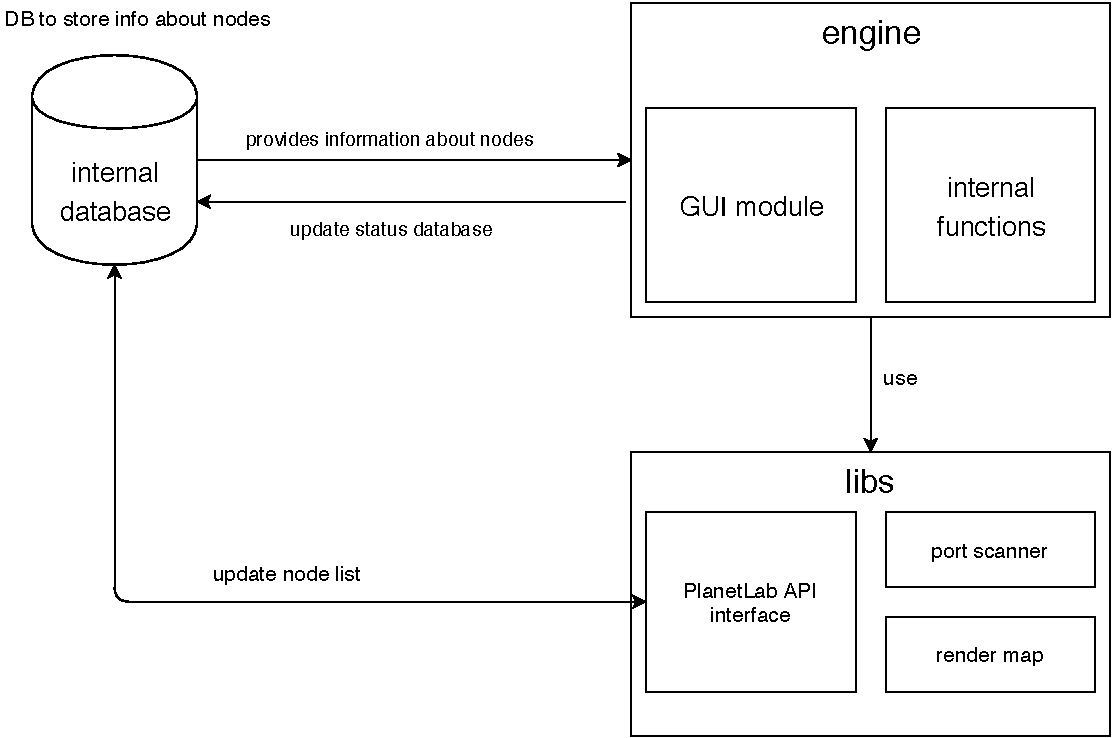
\includegraphics{obrazky/PlbmngArchitecture}}
	\caption{New PlanetLab Server Manager architecture diagram.}
	\label{fig:archdiagram}
\end{figure}

Issue with scattered functions was solved using single file, the \texttt{engine.py}, for all the common internal functions and graphic functions and libraries for more complex functionality of the application. To make it easier to navigate inside the engine file, it was divided between graphic and internal logic sections. A question why not to split the graphical and internal logic might come to a mind. Currently, the engine module graphical and internal functions are calling each other as an reaction to certain states. Splitting them would mean importing each other in a circle which is not an ideal state. Having both sections in one file makes it one solid logical component, called the engine. However as mentioned, there are certain independent components that are split into their own files. In the Figure~\ref{fig:archdiagram}, these are described as \texttt{libs} and contains several utility functions that can be called independently and are imported as a library inside the \texttt{engine}. Currently, there are three of these utility modules. PlanetLab API interface, which provides data for updating the application database of servers, port scanner which allows to check port accessibility of remote host and lastly module that allows to render map of nodes using a dictionary of nodes as input. On of the challenges during re-design was a placeholder for all the information about nodes that application can later used. Previously, a text file was used to store this data. Issue with this is to implement a filter function for example, it would require to write a custom module for queries which is an unnecessary overhead as there are already solutions available to provide such module. One of these solution is relational database with SQL used as a query language. SQL is a structured query language designed to manipulate data in relational tables which are nothing more than set of related information~\cite{Beaulieu:2005:LS:1098720}. This fits perfectly application needs as it stores a set of nodes with their related status information. In the Figure~\ref{fig:archdiagram}, this is shown as an internal database module. Engine triggers update of status of available nodes whereas PlanetLab API interface library updates the list of nodes. Python provides a \texttt{SQLite3} library that allows creating a custom database stored on disk. This database file is placed inside the database folder in the application configuration management. Mentioned architecture decisions will allow application to be more easily salable and maintainable in the later development phases.\\

\section{Description of Improvements}
\label{section:implementapproach}
In this Section, the steps to achieve goals--which were described in the Chapter introduction--will be shown in detail in their own Subsections. For each Subsection the approach, specific steps, code examples and results will be illustrated. Since the new implementation uses \texttt{pythondialog} module, at the start of the tool an instance of the \texttt{Dialog} class is spawned and will be later described just as the \texttt{instance}.
\subsection{Removal of Search Result Limitation}
The previous version of \texttt{plbmng} tool has been limited to 10 result while searching for a node. This issue was introduced due to difficulty of creating a menu based on dynamic results since author needed to always append another argument to the overall menu command. This approach can also hit limitation of characters that can be passed in a Bash command line. In Python~3 this problem does not exists since \texttt{pythondialog} module is creating menu functions based on \texttt{list}. During the search of nodes, results are added to the list which is after completed search passed to the instance which renders the \zk{zkGUI} (\zkratkatext{zkGUI}). Example of this functionality is shown in Listing~\ref{lst:removingresultlimit}. Due to this improvement tool is returning all results found.

{\noindent\begin{minipage}{\linewidth}
\begin{lstlisting}[language=Python, numbers=left, label={lst:removingresultlimit}, caption=Removing result limitation by passing choices as a list argument., frame=single, showstringspaces=false, keywordstyle=\color{blue},captionpos=b]
def searchNodesGui(prepared_choices):
	if not prepared_choices:
		d.msgbox("No results found.", width=0,height=0)
		return None
	while True:
		code, tag = d.menu("These are the results:",
							choices=prepared_choices,
							title="Search results")
\end{lstlisting}
\end{minipage}

\subsection{Writing the Application as Library}
For the application to be used in other scripts and to reduce need to re-write certain code parts it is desired to write application to be able to run as a library. During the re-implementation this was considered and application is available both as library and standalone script. This will be later used in the Subsection~\ref{section:improvement}. If the application is called as a standalone script it will trigger part of the code that is shown in Listings~\ref{lst:pythoninit} which will initialize graphical interface. If imported as a library, it allows the user to call any function defined in the script.

{\noindent\begin{minipage}{\linewidth}
\begin{lstlisting}[language=Python, numbers=left, label={lst:pythoninit}, caption=Condition to recognize that application is being called as a standalone script., frame=single, showstringspaces=false, breaklines=true, keywordstyle=\color{blue},captionpos=b]
if __name__ == "__main__":
	initInterface()
	exit(0)
\end{lstlisting}
\end{minipage}

\subsection{Code Readability Improvement}
\label{subsection:readability}
Community is a powerful group that helps develop a tool and to add more functionality to it. To have community contribute to a tool, it should follow good practices and be easily readable and understandable. Previous version of the tool was using Bash script which was calling Python script and creating new Bash scripts on a disk which was merging using different pieces of code from pre-created \texttt{.dat} files in a \texttt{bin} folder. Finding a bug in this structure was difficult and navigating was not intuitive. Most functions were fully re-written into single Python script and logically divided into two sections. One section is for GUI functions and other is for logical functions. Stand-alone functions were moved to a separated scripts to be used as a library. Each functions is very descriptive in its name as shown in Listing~\ref{lst:descriptive}.

{\noindent\begin{minipage}{\linewidth}
\begin{lstlisting}[language=Python, numbers=left, label={lst:descriptive}, caption=Example of Function Names, frame=single, showstringspaces=false, breaklines=true, keywordstyle=\color{blue},captionpos=b]
def searchNodes(option,regex=None):
def initInterface():
def plotServersOnMap(mode):
def getPasswd():
def searchNodesGui(prepared_choices):
def printServerInfo(chosenOne):
def setCredentialsGui():
\end{lstlisting}
\end{minipage}

Each functions is trying to be as atomic as possible only having one purpose. This is helping to increase modularity of the application. Outside of this function "categories" tool is removing any \texttt{magic numbers} by defining constants at the beginning of the source code. This greatly helps to understand what is being passed as an argument and is shown in Listing~\ref{lst:constant} where it is descriptive what option is being passed as a search key to the \texttt{searchNodes} function. Also, the application has a block for \texttt{Initial settings} at the beginning for one single place where outside of functions definitions can be placed. Application is also honoring the conventions defined in \zk{zkPEP} (\zkratkatext{zkPEP}) 8 \cite{pythonpep}, like naming convention and space usage instead of tabs, as much as possible. In default, scripts like \texttt{pylint} uses snake case style naming convention however camel case that is actually described in the official pep 8 standards as a recommended descriptive naming style \cite{pythonpep}. All these small items described are increasing the overall readability of the application for others to quickly become familiarized with it. Currently, main script \texttt{engine.py} received score of 7.38  \texttt{pylint} with main complains being about missing doc strings and certain minor warnings regarding wrong import and other small deviation from the PEP 8 standard.

{\noindent\begin{minipage}{\linewidth}
\begin{lstlisting}[language=Python, numbers=left, label={lst:constant}, caption=Example of Constant Usage, frame=single, showstringspaces=false, breaklines=true, keywordstyle=\color{blue},captionpos=b]
code, tag = d.menu("Choose one of the following options:",
					choices=[("1", "Serach by DNS"),
				      		 ("2", "Search by IP"),
					    	   ("3", "Search by location")],
						       title="ACCESS SERVERS")
if code == d.OK:
	#Search by DNS
	if(tag == "1"):
		code, answer = d.inputbox("Search for:",title="Search")
		if code == d.OK:
			searchNodes(OPTION_DNS,answer)
		else:
			continue
\end{lstlisting}
\end{minipage}

As mentioned in the Section~\ref{section:improvement}, renaming certain parts of the tool can improve the readability. Since the tool is not data mining rather than server manager, the tool is renamed from \texttt{Data miner or PlanetLab} into \texttt{PlanetLab Server Manager}. Version is added next to the name for users to see which they are running immediately. Another example is renaming \texttt{Search nodes} to \texttt{Access servers} since primary function of this menu item is to access the servers while search is just supporting it. The re-designed application can be seen in Figure~\ref{fig:redesigned}.\\

\begin{figure}[H]
	\centering
	\scalebox{0.58}{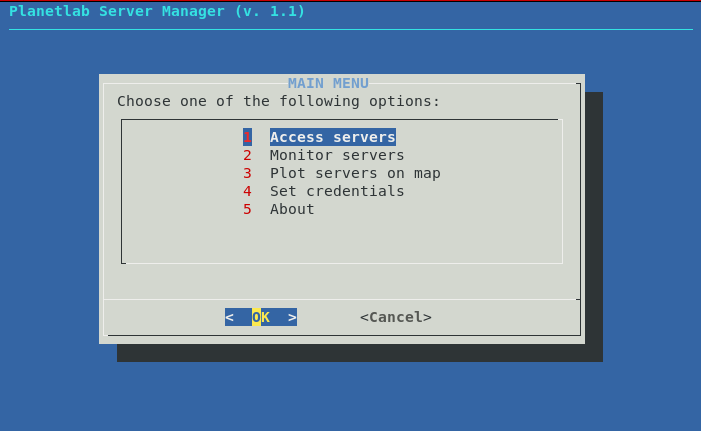
\includegraphics{obrazky/plbmng_basic}}
	\caption{Re-designed menu of new PlanetLab Server Manager.}
	\label{fig:redesigned}
\end{figure}

\subsection{Removal of Pre and Post Installation Steps}
Previous version of application required several pre and post installation steps. In the new version developed as part of this Diploma thesis, all these steps were removed. Pre-installation steps were eliminated by completely getting rid of dependencies on additional system packages. All dependencies were moved into the PyPI package definition and are taken care off PyPI installer during installation of the tool. Post-installation steps were removed by adding the application into \texttt{bin} folder in the PyPI package. During installation, the PyPI installer automatically puts any scripts in the \texttt{bin} folder into a \texttt{\$PATH} folder making it accessible directly from command line without the need of accessing installation folder. The contents of the main, but simple, script located in \texttt{bin} folder can be seen in Listing~\ref{lst:plbmngbin}.

{\noindent\begin{minipage}{\linewidth}
\begin{lstlisting}[language=Python, numbers=left, label={lst:plbmngbin}, caption=Source code of the main script populated by PyPI installer into executable folders., frame=single, showstringspaces=false, breaklines=true, keywordstyle=\color{blue},captionpos=b]
#! /usr/bin/env python3
from plbmng import engine
import sys

if len(sys.argv) > 1:
	if(str(sys.argv[1]) == 'crontab'):
		engine.updateAvailabilityDatabaseParent('cron')
		exit(0)

engine.initInterface()
\end{lstlisting}
\end{minipage}}

\subsection{Improvement of Credentials Management}
In the previous version of the tool the credentials were filled using \texttt{dialog} forms. When typing the credentials, nothing was shown except stars thus user was unaware where is the position of the cursor. Also saving the credentials was not working properly resulting into the need to adjust the configuration file on the disk which required locating the file first by inspecting the source code. In the new version settings credential is improved by creating a virtual editor in the graphical interface itself, as shown in Figure~\ref{fig:credentials}, which allows the user transparently set the credentials. One of the disadvantage of this approach is plain text visible password in the editor as it is not hidden and user needs to be careful about setting the credentials in a safe environment. To the addition of this improvement, various credentials checks were added to the application. First run of the tool will always trigger pop-up window advising user to fill credentials first. If a user chose to update a database without having credentials filled a warning message will pop-up warning the user about that fact. Also, when user wants to ssh to a server without having username and key filled he will have warning text near the ssh option. These improvements should prevent users forgetting about filling credentials and failing actions in the application.

\begin{figure}[H]
	\centering
	\scalebox{0.5}{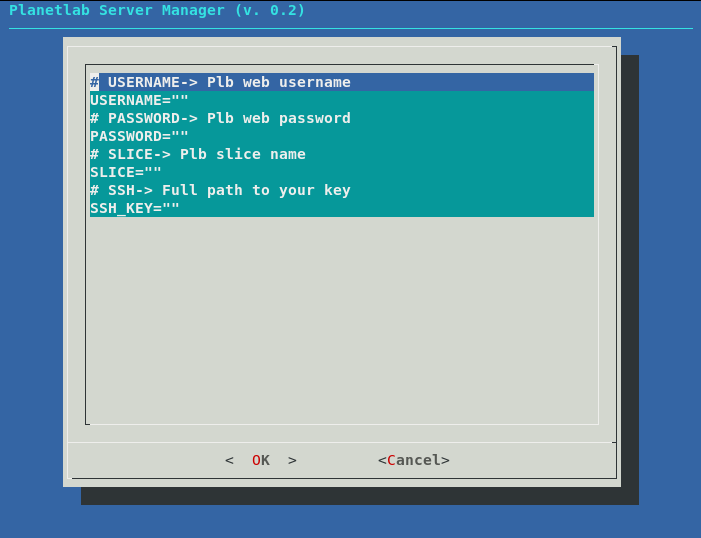
\includegraphics{obrazky/credentials_figure}}
	\caption{New window for setting up credentials using internal text editor.}
	\label{fig:credentials}
\end{figure}

\subsection{Application Folder Structure Re-design}
With changes to the architecture of the application, folder management needs to be also adjusted accordingly. The root folder of the application contains two main parts, outside of necessary PyPI files. It is the \texttt{bin} folder with \texttt{plbmng} script itself and the \texttt{plbmng} folder which contains the whole application logic and graphical interface. This folder will be now described in detail. As characterized in Section~\ref{section:redesign}, libraries are placed in the \texttt{lib} folder instead of \texttt{python\_scripts} previously. In past, the configuration files were stored in \texttt{bin} folder with shell scripts. This has been re-named to \texttt{conf} folder and library functions were moved to the \texttt{lib} folder. There are information that needs to be stored persistently, like information about accessibility of nodes. For this purposes, there is a folder called \texttt{database} which contains file like \texttt{internal.db} which is already mentioned \texttt{SQLite3} database. With all these changes to the folder structure, the project should be now more transparent, clear and easier for other developers to join the project.

\subsection{Filtering Nodes Based on Accessibility}
One of the goals if this Diploma thesis was to add a functionality to filter nodes based on their accessibility. This Subsection will describe how the functionality was designed and implemented. The overall idea was to add a way to filter current node based on their availability, have an option to change these settings, show these settings and have a way to update the data. In the following paragraph, all these items will be described more in detail.\\
As it was mentioned in Section~\ref{section:redesign}, the core of this functionality was to have a placeholder for the data about the nodes. This was achieved using the \texttt{SQLite3} Python library. To store the information, table \texttt{availability} was created and its structure can be seen in Table~\ref{table:availability}. First, \texttt{nkey} column is a primary key column that contains ID of the table row. Next is \texttt{shash} that contains unique hash of the node hostname. This hash is used to find already existing records so these are not duplicated but only updated. Hash is generated using md5 function and \texttt{hashlib} Python library. Next column is a \texttt{hostname} of the node for purposes of filtering and lastly there is the double \texttt{bssh} and \texttt{bping} which are Boolean flag displaying node accessibility. During insert into the database, \texttt{nkey} is automatically incremented thus only other values needs to be specified. Before the filtering is explained, first the internal logic working with nodes needs to be characterized. When an user select to display nodes, the search function takes a dictionary of nodes as an input parameter. This simple logic is used for the filtering itself. In the function \texttt{getNodes()}, before the list of nodes is parsed, the current settings are loaded from the database from the \texttt{configuration} table which contains simply ID, name of the setting and Boolean if it is enabled or not. These settings are used to get all hostnames of the nodes that fits the current settings. For example, if user wants to filter only ssh available nodes, the query will be \texttt{select * from availability where bssh='T'}. With the list of desired nodes the function will always return only nodes that fits user's filter criteria.\\

\begin{table}[htb]
	\resizebox{\textwidth}{!}{\begin{tabular}{|l|l|l|l|l|}
			\hline
			\rowcolor[HTML]{EFEFEF} 
			nkey & shash                            & shostname                                & bssh & bping \\ \hline
			2    & fe27ca7d1707e86e1739b1819743dc79 & planetlab2.fri.uni-lj.si                 & F    & F     \\ \hline
			3    & 57da801bf4370f2a163a81bdf6bafa8c & ple01.fc.univie.ac.at                    & T    & F     \\ \hline
			4    & 3c956d5e295f17cb303773f83c84bf17 & aladdin.planetlab.extranet.uni-passau.de & T    & T     \\ \hline
		\end{tabular}
	}
\centering
\caption{Structure and examples of availability table for filtering functionality.}
\label{table:availability}
\end{table}

Applying filters is done using \texttt{Filtering options} in the \texttt{Access servers} menu. As shown in Figure~\ref{fig:filtering}, user can choose between ssh or ping available nodes. The selection is done using checkboxes. The choices are then shown in the  \texttt{Access servers} menu on the top as \textit{Active filters} line with the listing of the active options. \\

\begin{figure}[H]
	\centering
	\scalebox{1}{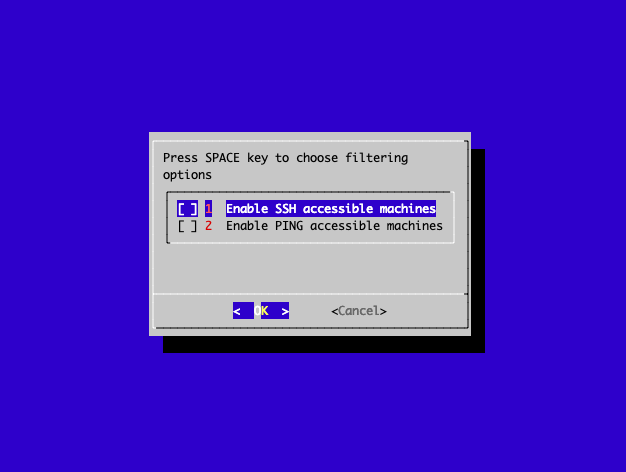
\includegraphics{obrazky/filtering}}
	\caption{Figure showing new menu where user can choose active filters.}
	\label{fig:filtering}
\end{figure}

\subsection{Multiprocessing Update of Status Database}
Updating the status database, or to be precise updating table inside the database, can be triggered from the \texttt{Monitor servers} menu. This will start a progress bar that takes approximately two minutes after optimization. Before optimization, the procedure took around 40 minutes. This speed was reached using multi-processing. Once procedure to update database is triggered, fifty processes are spawned at a same time using Python \textit{multiprocessing} library. List of nodes is passed as an iterator to go over in a loop to the \texttt{Pool} object as shown in Listing~\ref{lst:multiprocess}. In addition, one lock is created to take over critical section of updating the shared status database and progress bar. Critical section can be defined as an area in a computer program where process operates on the shared variable by changes its value \cite{gebali2011algorithms}. Once a process reaches the critical section, it needs to acquire the lock to enter into it. Once a process has acquired the lock, it can start writing into the shared memory without any issue. As soon as it is done, the lock is released and another process can acquire it and start writing into the critical section. To be able to show correctly the progress, once a process finishes a task, it will lock the progress bar value, increase the progress variable with an increment that is derived from total number of nodes and then unlock the progress bar iterating to another node to gather information about it. The code of entering the critical section can be seen in  Listing~\ref{lst:lock}\\
 
{\noindent\begin{minipage}{\linewidth}
		\begin{lstlisting}[language=Python, numbers=left, label={lst:multiprocess}, caption={Creating a multi-processing object with fifty processes, three shared variables and list of nodes as iterator.}, frame=single, showstringspaces=false, breaklines=true, keywordstyle=\color{blue},captionpos=b]
pool = Pool(50, initializer=multiProcessingInit,
		  	initargs=(lock,base,increment, ))
pool.map(updateAvailabilityDatabase, nodes)
		\end{lstlisting}
	\end{minipage} 

{\noindent\begin{minipage}{\linewidth}
		\begin{lstlisting}[language=Python, numbers=left, label={lst:lock}, caption=Entering a critical section and acquiring lock., frame=single, showstringspaces=false, breaklines=true, keywordstyle=\color{blue},captionpos=b]
lock.acquire()
base.value = base.value = increment.value
updateProgressBarMultiProcessing(base.value)
lock.release()
		\end{lstlisting}
	\end{minipage} 

\subsection{Improvements of Node Visualization}
In the previous version of the application, user could render all nodes in the node database on a map. It displayed markers which, upon clicking, showed hostname of the node. During implementation of filters, maps were also enhanced. Now, user can select between three maps to render; full map, map of nodes available over ssh and map of nodes that are ping-able. In addition, upon clicking, user can see all the stored information about the node as can be seen in Figure~\ref{fig:mapnodedetail}. The library for rendering the map was changed to use the same principle as search function. Instead of reading nodes from a file, it gets them passed as a parameter. While triggering the map module, nodes are loaded using \texttt{getNodes()} function that takes filtering into consideration in default. The filter in this case is only adjusted by the user's choice. Later, in Section~\ref{section:analysis} the information from map filters will be used to analyze \textit{PlanetLab Network} more in detail. For user, maps filters are good opportunity to see which server are actually available for project testing and possibly create an uniform list of candidate nodes that are spread all over the world. 

\begin{figure}[H]
	\centering
	\scalebox{0.65}{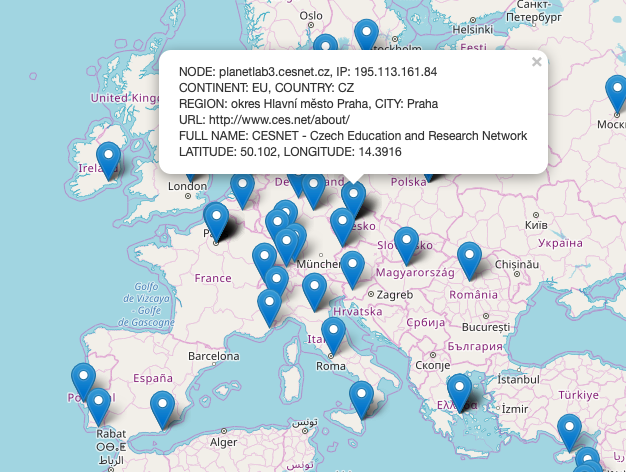
\includegraphics{obrazky/mapnodedetail}}
	\caption{Detail of node marker with newly added information about the particular node \cite{OpenStreetMap}.}
	\label{fig:mapnodedetail}
\end{figure}

\subsection{Minor Improvements}
In this Subsection, minor improvements done during the re-implementation are described. All these improvements were considered minor hence they do not have separate Subsection.
\paragraph{Clearing of the screen after cancel}
When signal was send to the application using \texttt{CTRL + C} key combination, the previous version of the application was not clearing the current terminal window and the GUI. To use the same terminal user was forced to clear the window manually. In the new version, when signal is send to the application, signal handler will catch it and clean after itself.
\paragraph{Recursion removal for return}
When returning from child window to a parent page, the previous version of application was recursively calling the GUI function. This is not following good coding habits as each recursive call means storing the previous function details into the system stack, unnecessarily filling it. In the new version, while cycle is used instead and returning from a function results into new iteration of the while cycle not storing anything onto the system stack. 
\paragraph{About is added to the menu}
About section is added to the menu displaying version, authors and the license.
\paragraph{Crontab mode created}
Application has option to run with \texttt{crontab} argument which will trigger just monitoring of the nodes. This is in particular useful when setting the \texttt{crontab} since the call can be simply \texttt{plbmng crontab}. This mode can be used to setup a regular updates in background to the node database.
\paragraph{Last server access}
User has now ability to return to last accessed server it the \texttt{Access servers} menu. In default, this option will just print warning message that no node was accessed. However, as soon as user access first node, this node is stored into the database in form of dump of the node dictionary variable. If user wants to access the last accessed node, this dictionary is dumped back to an internal variable and used to show this node with all the information and options.
\paragraph{Menu with statistics}
Since status database already contains all the necessary information a simple functionality regarding accessibility of the stored nodes was added to the application as can be seen in Figure~\ref{fig:statmenu}. 

\begin{figure}[H]
	\centering
	\scalebox{1}{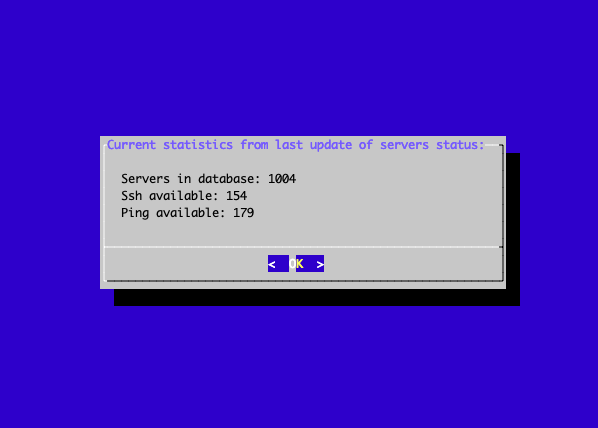
\includegraphics{obrazky/statmenu}}
	\caption{Newly added option to display current statistics about accessibility of stored nodes.}
	\label{fig:statmenu}
\end{figure}

\paragraph{Support of Multiple Platforms}
As was mentioned previously, Python is multi-platform language and brings possibility of porting the application to all kinds of different operating systems. During the re-implementation of the application this was taken into considerations and new functions were written to be able to run on Linux, Mac and possibly later on even Windows. Example of this multi-platform implementation can be seen in Listing~\ref{lst:testping} showing function \texttt{testPing} supporting all mentioned operating systems. As both Linux and Mac are Unix based, the implementation for these operating system is fairly simple and only minor changes are usually in several parameters. Good example is \texttt{ping} function. On Mac, time-out parameter takes one integer in millisecond as input variable. However, on Linux, the time-out parameter takes the integer variable in seconds. These little differences needs to be kept in mind when implementing platform-based functions. For Windows however, the differences are even more complex and all the libraries used in \texttt{plbmng} have to have Windows support. This was never tested yet even though most of the functions were written with Windows in mind. Adding full Windows support is a good initiative for the future development of \texttt{plbmng}.

{\noindent\begin{minipage}{\linewidth}
		\begin{lstlisting}[language=Python, numbers=left, label={lst:testping}, caption={Example of fully multi-platform function testPing.}, frame=single, showstringspaces=false, breaklines=true, keywordstyle=\color{blue},captionpos=b]
def testPing(target, returnbool=False):
	pingPacketWaitTime = None
	if system().lower() == 'windows':
		pingParam = '-n'
	else:
		pingParam = '-c'
	#for Linux ping parameter takes seconds while MAC OS ping takes miliseconds
	if system().lower() == 'linux':
		pingPacketWaitTime = 1
	else:
		pingPacketWaitTime = 800
	command = ['ping', pingParam, '1', target, '-W', str(pingPacketWaitTime)]
	p = subprocess.Popen(command, stdout=subprocess.PIPE,
	stderr=subprocess.PIPE)
	# prepare the regular expression to get time
	if system().lower() == 'windows':
		avg = re.compile('Average = ([0-9]+)ms')
	else:
		avg = re.compile(
		'min/avg/max/[a-z]+ = [0-9.]+/([0-9.]+)/[0-9.]+/[0-9.]+')
		avgStr = avg.findall(str(p.communicate()[0]))
	if p.returncode != 0:
		if not returnbool:
			return "Not reachable via ICMP"
		return False
	else:
		p.kill()
		if not returnbool:
			return avgStr[0]+" ms"
		return True
		\end{lstlisting}
	\end{minipage}

\subsection{Minor Bug Fixes}
In this Subsection, minor bug fixes will be described which were not considered as enough improving to be included in separate Subsection. 
\paragraph{Removing headers from the searches}
During the search, previous version of the script has also included header of the file containing information about nodes resulting into false search results. Header is now skipped and these false results are removed.
\paragraph{Application crashes during return}
When returning from a child menu window to a parent page, the application tend to crash on \texttt{grep} tool not being able to find file. During re-implementation this bug was fixed and returning now fully works.

\section{Improved Installation and Use of Application}
\label{section:currentapp}
In this Section, the post-improvements installation procedure is described and workflow diagram is shown in Figure~\ref{fig:workflowdiagram}. After implementing improvements, application has been updated in the PyPI repository and is available at \url{https://pypi.org/project/plbmng/} in version \texttt{0.3.7}. Application repository web page can be seen in Figure~\ref{fig:plbmngrepo} and is describing the tool purpose, its Python package dependencies, installation steps, basic usage and authors. Repository page gives ability to the user to see release history or download the source files of the project. It also show the maintainers of the projects and allows users to contact them. License under which the application is written can be found the repository page as well. As part of this Diploma thesis, the description was changed to reflect the current settings. It was improved to be more simple for the user by reducing amount of text on the page and keeping only necessary information.

\begin{figure}[H]
	\centering
	\scalebox{0.38}{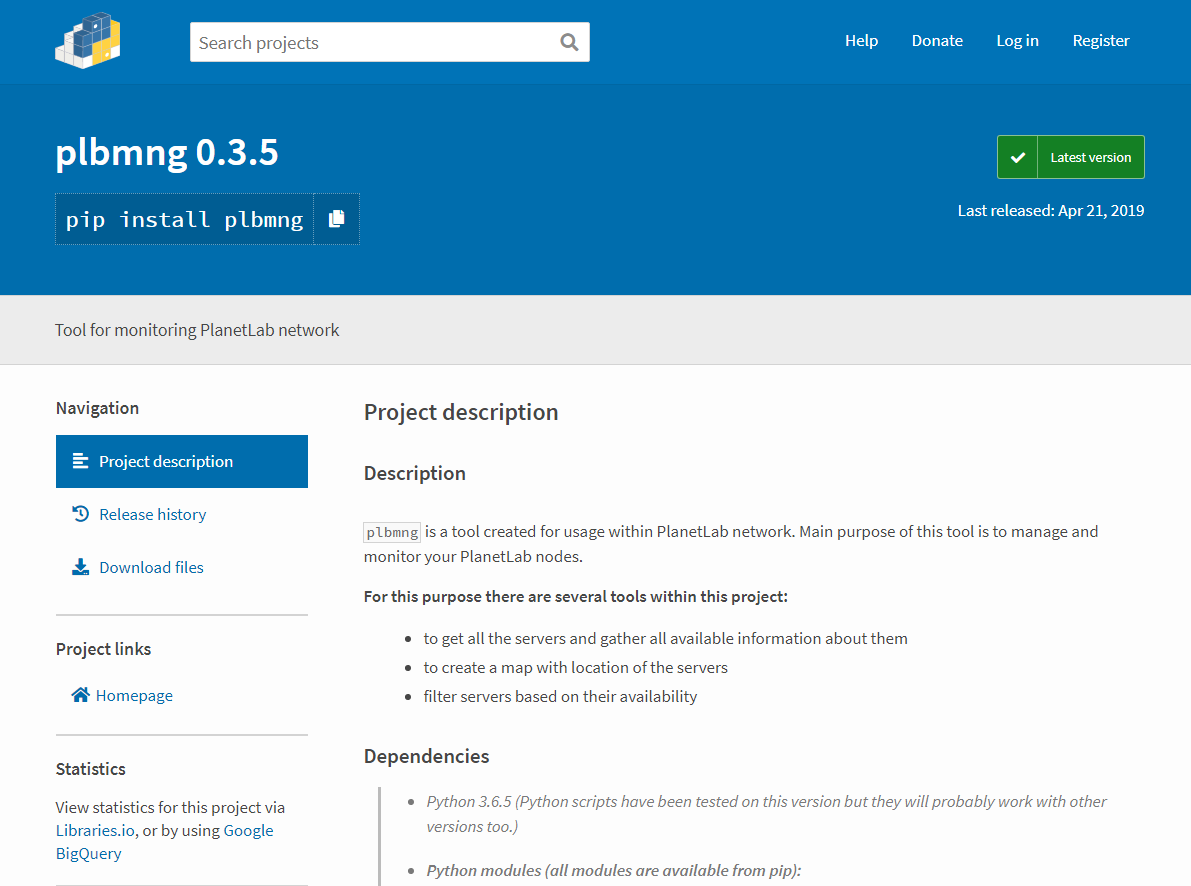
\includegraphics{obrazky/plbmng_repo}}
	\caption{New PlanetLab Server Manager web page in PyPI repository.}
	\label{fig:plbmngrepo}
\end{figure}

The installation steps are described in detail in the tool's repository page and consist of:

\begin{enumerate}
	\item Installing the application using \texttt{pip3 install plbmng} command.
	\item Starting the application using \texttt{plbmng} command.
	\item In first start it is required to set up credentials using the \texttt{Set credentials} option in menu.
\end{enumerate}

After this basic setup all the application functionality is available. It is recommended though, to update the list of nodes using \texttt{Get nodes} option in \texttt{Monitoring} menu. Installation steps are successfully reduced compared to the previous version which consisted of:

\begin{enumerate}
	\item Installing system packages using \texttt{sudo dnf install -y dialog pssh fping} command.
	\item Installing the application using \texttt{pip install plbmng} command.
	\item Locating the application in a hidden folder of pip tool.
	\item Finding a configuration file and using an editor to update it.
	\item Running the application using absolute path.
\end{enumerate}

\paragraph{} To summarize, current application functionality workflow diagram can be seen in Figure~\ref{fig:workflowdiagram}. For sake of diagram readability, the Figure~\ref{fig:workflowdiagram} is missing returning arrows however each node in the diagram is able to return to its parent. As seen in the Figure, first step is when menu is being initialized. From there user has option to either open \texttt{Access server menu}, \texttt{Monitor servers}, \texttt{Plot servers on map}, \texttt{Set credentials}, \texttt{About} or select \texttt{Statistics}. \texttt{Statistics} will display current data about nodes accessibility. \texttt{About} is a single window option that will show information about the software, its authors and license. \texttt{Set credentials} option will open an interactive editor where user can fill the credentials for PlanetLab network. Next option is \texttt{Plot servers on map} which offers user to choose which map elements should be displayed. After confirmation the map is generated and opened in the system default browser. \texttt{Monitor servers} option divides into three different options. First enables user to setup \texttt{crontab} to periodically scan for new nodes, second option is for updating status database and third updates list of nodes. At last, \texttt{Access servers} allows users to access the nodes by searching for them either using DNS name, IP address or location. After the search key is inserted, the available results are shown. It also offers user to get to last accessed node or select filtering option which are displayed on the top of the window. When specific node is chosen, information about the node are displayed and user has options to connect to the node using ssh, Midnight Commander or show the node on map. If credentials are not filled, warning message next to option is displayed.

\begin{figure}[H]
	\centering
	\scalebox{0.8}{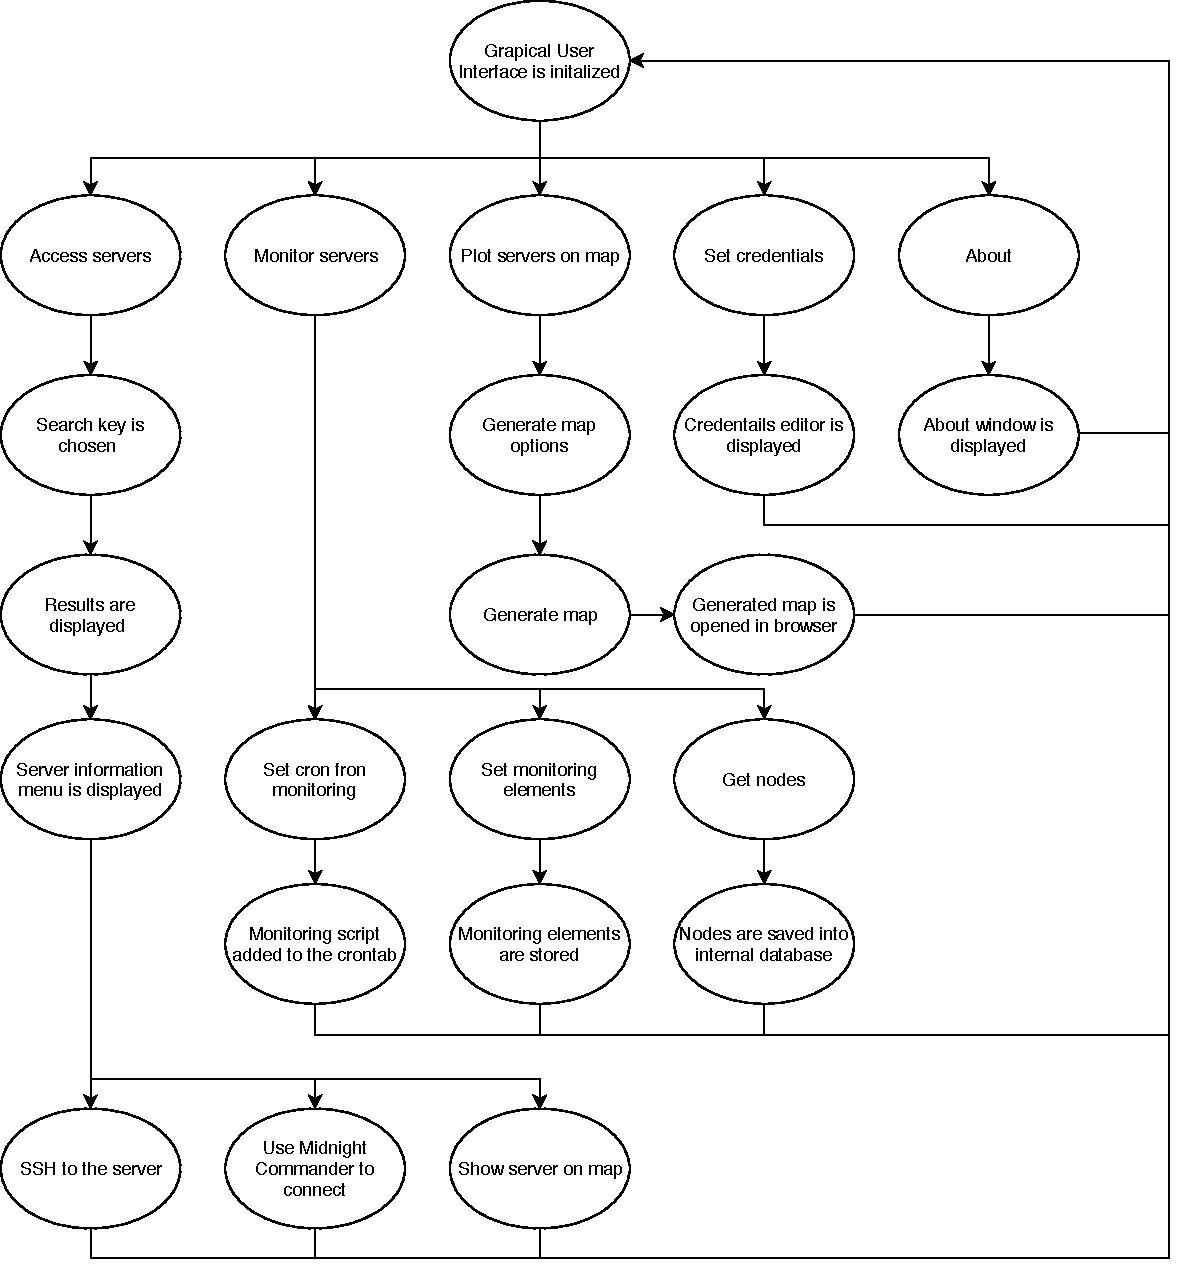
\includegraphics{obrazky/BehavioralPlbmng}}
	\caption{Behavioral diagram of new PlanetLab Server Manager.}
	\label{fig:workflowdiagram}
\end{figure}

\chapter{PlanetLab Server Manager Use Cases}
\label{chapter:usecase}
In this Chapter, various use cases of the PlanetLab Server Manager tool will be revised and described. First, analysis of the PlanetLab Network will be done in Section~\ref{section:analysis}. In Section~\ref{section:testing}, the very basic use case of the application, testing network projects in the PlanetLab Network, will be described and shown.

\section{PlanetLab Network Analysis Using Plbmng Tool}
\label{section:analysis}
In this Section, the Planet Lab network will be analyzed and discussed using the newly developed features plus using the \texttt{plbmng} database of servers pulled from the PlanetLab API. Also, data from Chapter~\ref{chapter:planetlabnetwork} introduction will be compared to new ones with time difference of five months.\\
PlanetLab Network is a huge project which consists of 1353 nodes at 717 sites \cite{planetlabmain}. Currently, there are around one thousand servers available to the \textit{cesnet\_utko} user from 52 countries world wide. The Figure~\ref{fig:allcountriesgraph} shows 20 countries, represented by their country code, with the most node contribution to the network which X axis showing the country and on the Y axis showing the node count for the specific country. Most of the countries are from United States with the impressive node count of 388, second is China with its 58 nodes and third is Germany with their 49 nodes. 

\begin{figure}[H]
	\centering
	\scalebox{0.44}{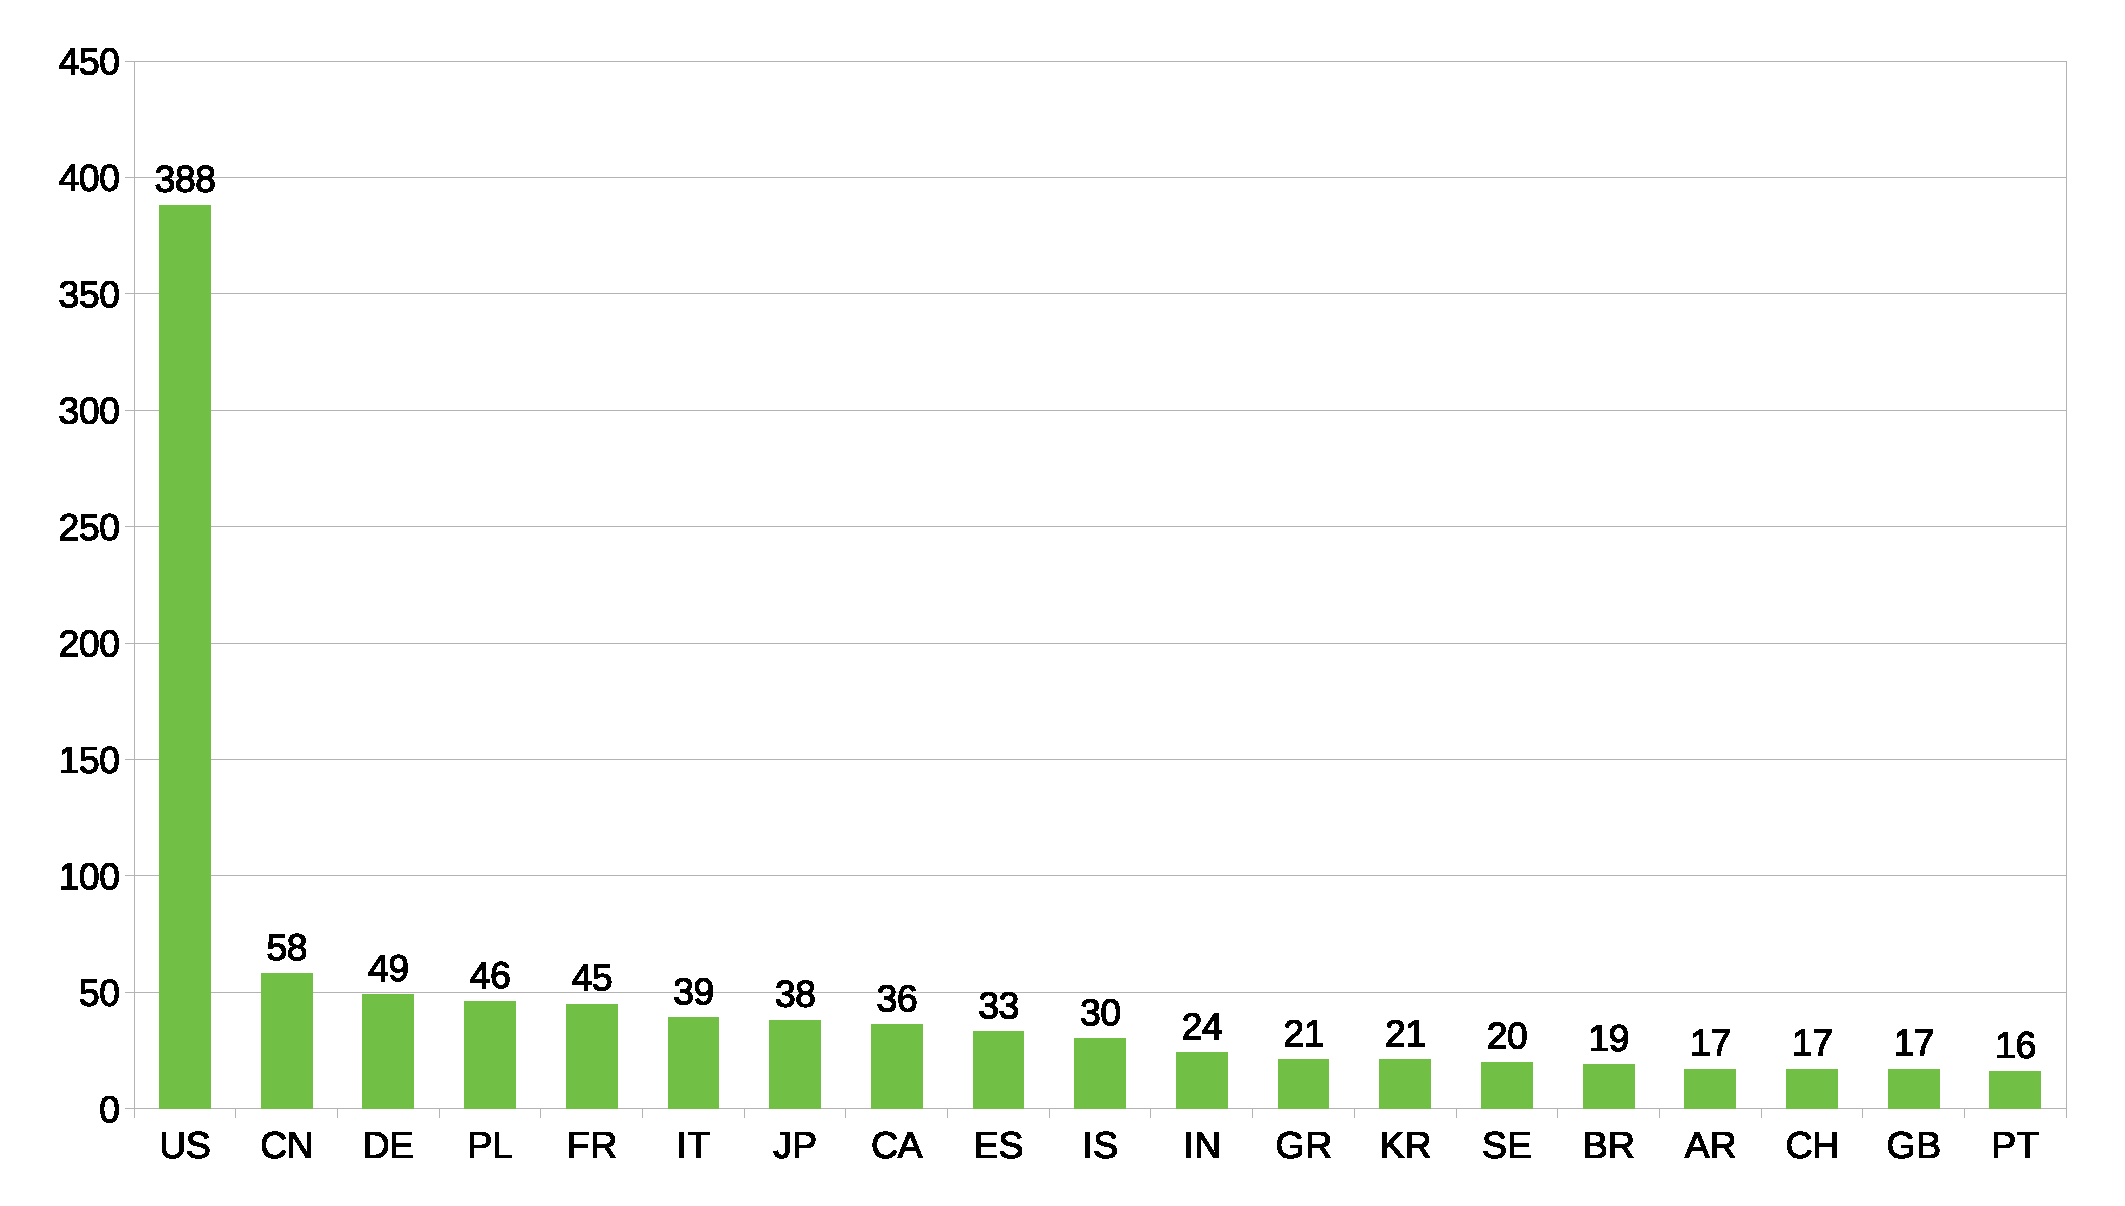
\includegraphics{obrazky/allcountriesgraph}}
	\caption{Graph displaying top twenty countries and number of nodes they have contributed to the PlanetLab Network.}
	\label{fig:allcountriesgraph}
\end{figure}

Geographically, the nodes are all over the world and are more then suitable to test large scale network project requiring multiple servers in different locations all over the world. All the nodes on a world map can be seen in Figure~\ref{fig:allnodes} which was created using \texttt{plbmng} application.

\begin{figure}[H]
	\centering
	\scalebox{0.55}{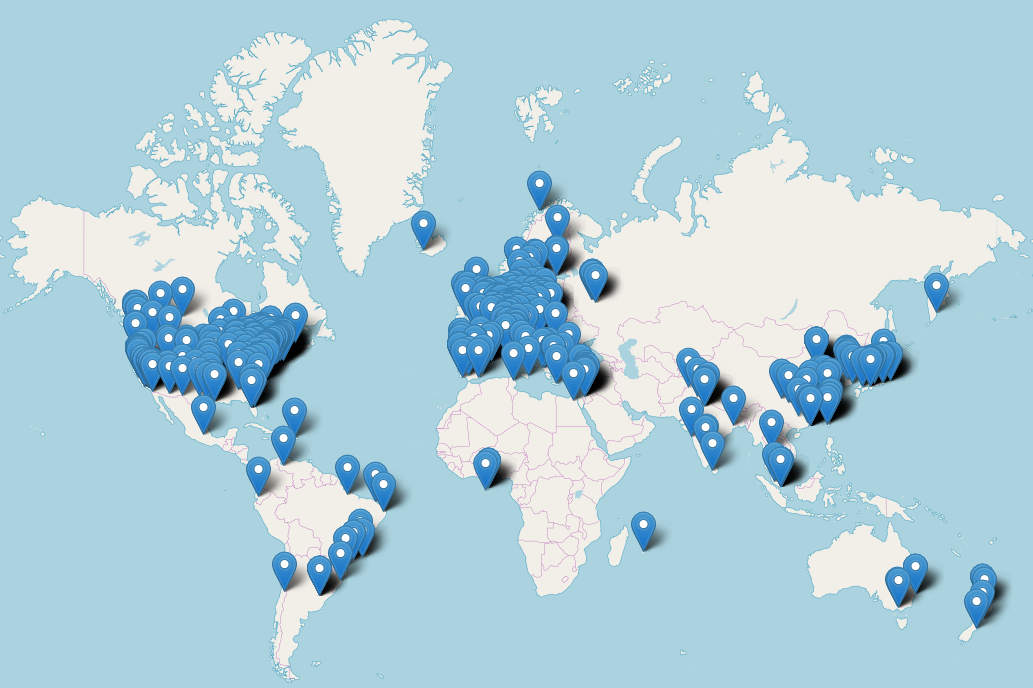
\includegraphics{obrazky/plbmng_all_nodes}}
	\caption{Nodes displayed on world map using the PlanetLab Server Manager map rendering functionality \cite{OpenStreetMap}. Data from April 2019.}
	\label{fig:allnodes}
\end{figure}

However, not all the nodes are available. As seen in Figure~\ref{fig:nodestats}, from the database 1004 nodes only 168 nodes are responding to ICMP packets and only 140 are listening on port 22 which is usually used for ssh. That is a very low availability percentage of only \SI{16.7}{\percent} nodes responding to ping and even less \SI{13.9}{\percent} listening on port 22. Interesting is also that 28 nodes stopped responding to ICMP packets since last measurement done in November 2018 as seen in Figure~\ref{fig:pingablepie}. That is extremely low number of available nodes and shows that the universities that are offering their nodes often do not maintain them to make sure these are still available or have left the project without decommissioning the node in the PlanetLab interface. Also, an interesting fact is that there are 28 nodes that are responding to ICMP packets but are not listening on port 22. Explanation can lie in stuck \texttt{sshd} agent or some network restrictions which are preventing to access the port 22 on specific server.

\begin{figure}[H]
	\centering
	\scalebox{0.95}{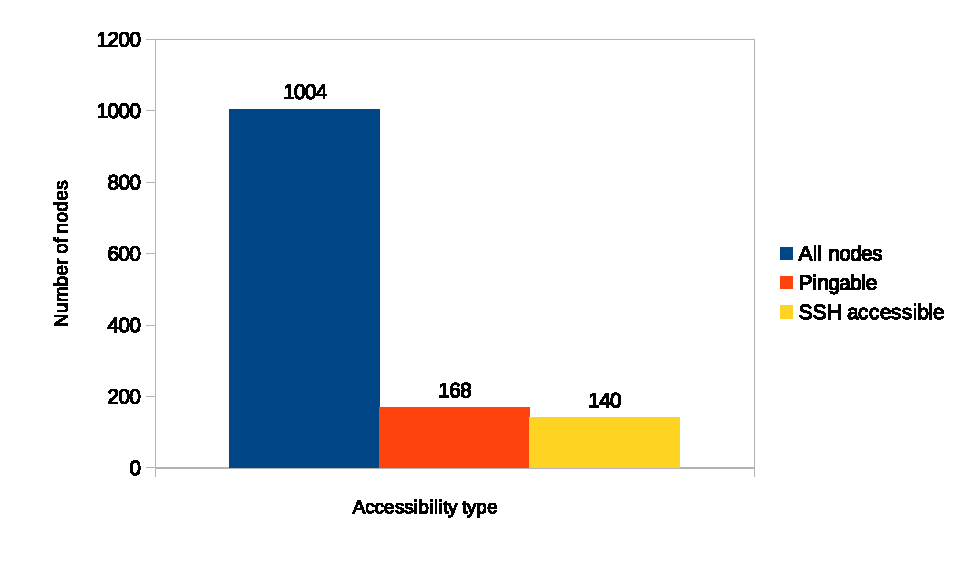
\includegraphics{obrazky/nodestats}}
	\caption{Number of PlanetLab nodes logically divided by their accessibility. Data from April 2019.}
	\label{fig:nodestats}
\end{figure}

If data are divided by continents, we will get graph with \texttt{ssh} accessible nodes in Figure~\ref{fig:sshcountriesgraph}. On the X axis, you can see continents and on the Y axis you can see number of accessible nodes on that particular continent. For Europe and America, the numbers are very similar. Interesting is that from South America, only 6 nodes are accessible and all are from Brazil.

\begin{figure}[H]
	\centering
	\scalebox{0.95}{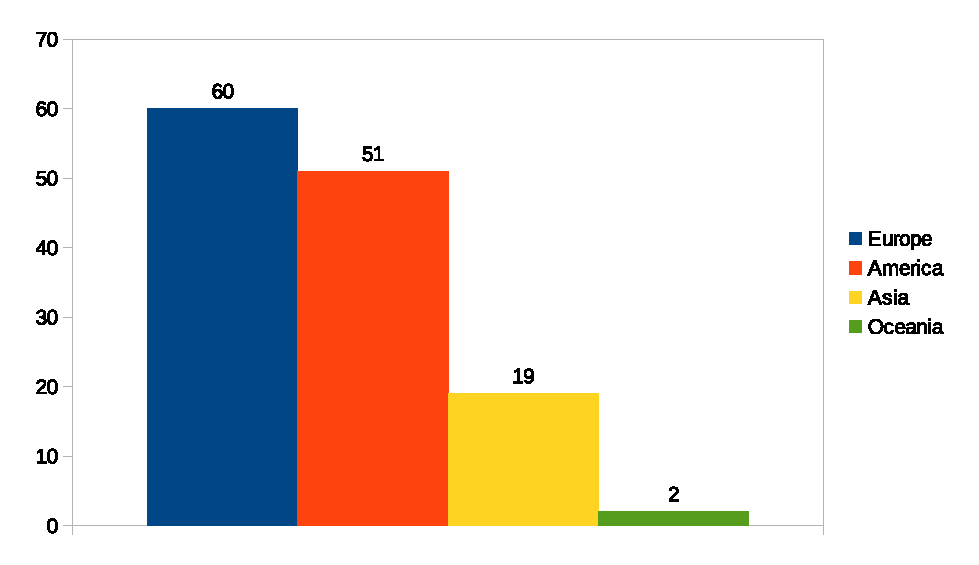
\includegraphics{obrazky/sshcountriesgraph}}
	\caption{Number of ssh accessible nodes logically divided into continents.}
	\label{fig:sshcountriesgraph}
\end{figure}

In more detailed breakdown, that can be seen in  Table~\ref{table:continentavailability}, it can be observed that Europe, with its \SI{12}{\percent}, has the biggest percentage of ssh-accessible servers compared to overall number of nodes of all continents. Ssh accessible node means node available for project testing. On the other hand, the lowest percentage of available server has China with only \SI{10.7}{\percent}.

\begin{table}[htb]
		\resizebox{\textwidth}{!}{
				\begin{tabular}{|c|c|c|c|c|c|c|c|}
					\hline
					\rowcolor[HTML]{C0C0C0} 
					\multicolumn{2}{|c|}{\cellcolor[HTML]{C0C0C0}Europe} & \multicolumn{2}{c|}{\cellcolor[HTML]{C0C0C0}America} & \multicolumn{2}{c|}{\cellcolor[HTML]{C0C0C0}Asia} & \multicolumn{2}{c|}{\cellcolor[HTML]{C0C0C0}Oceania} \\ \hline
					\rowcolor[HTML]{EFEFEF} 
					All nodes              & Ssh accessible              & All nodes              & Ssh accessible              & All nodes             & Ssh accessible            & All nodes              & Ssh accessible              \\ \hline
					332                    & 60                          & 422                    & 51                          & 177                   & 19                        & 18                     & 2                           \\ \hline
					\SI{100}{\percent}                  & \SI{18.6}{\percent}                      & \SI{100}{\percent}                  & \SI{12}{\percent}                        & \SI{100}{\percent}                 & \SI{10.7}{\percent}                    & \SI{100}{\percent}                  & \SI{11.1}{\percent}                      \\ \hline
				\end{tabular}
		}
\centering
\caption{Table comparing number of all nodes versus ssh accessible nodes per continent using plbmng status database.}
\label{table:continentavailability}
\end{table}

When map with all nodes, seen in Figure~\ref{fig:allnodes}, is compared to map with only ssh accessible nodes, seen in Figure~\ref{fig:sshnodes}, the difference is even more clear. Map rendering functionality can be used to plan project testing and offers filtering only ssh available nodes.

\begin{figure}[H]
	\centering
	\scalebox{0.55}{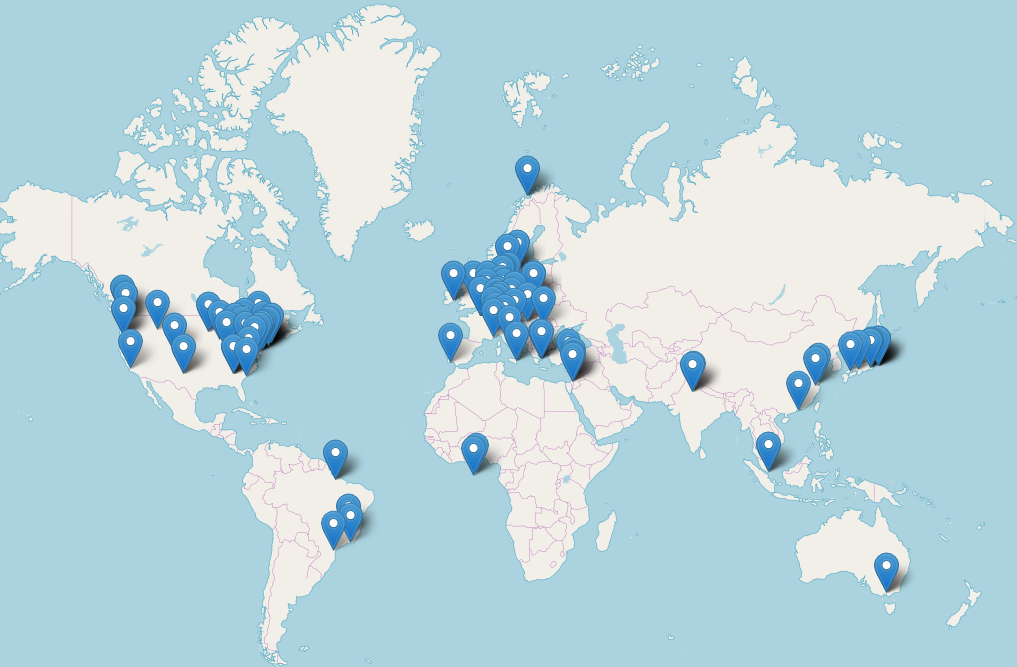
\includegraphics{obrazky/plbmng_ssh_nodes}}
	\caption{World map displaying only ssh-accessible nodes using application database \cite{OpenStreetMap}. Data from April 2019.}
	\label{fig:sshnodes}
\end{figure}


\section{Testing Network Projects with Planet Lab Server Manager}
\label{section:testing}
In this Section, a use case of testing a network projects, on of the most crucial use cases, will be shown and illustrated. For the purpose of illustration a simple imaginary project of running a listener on port 8765 in America and accessing it from China and Europe will be described. The idea of the project is to record the times that are required to establish a connection and log necessary turn-around time for a packet to travel between continents. Mentioned project is basically a simple implementation of \texttt{ping} tool.\\
As a first step, credentials needs to be updated in the \texttt{Set credentials} menu options. Next, filter is turned on to show only ssh accessible servers in the \texttt{Access servers} menu section. Later, a server is found using the \texttt{Search by location} menu option and credentials are verified. If the connection is successful, testing can continue. For this purposes, simple Python script will be used. There will be a server as seen in Listings~\ref{lst:echoserver} and client as seen in Listings~\ref{lst:echoclient} which all are inspired from \texttt{cyberciti.biz} site \cite{ports}. Server will be listening on port 8765 address 0.0.0.0 and client will send a packet with message "\texttt{Test successful.}" that will be send back to the client from the server as an echo reply. The results can be seen in Figure~\ref{fig:testingusecase} where, in the terminal, three consecutive runs of plbmng application were started and using the filter and \texttt{Search by location} menu option the ssh available servers from America, China and Europe were found and connected into. On the bottom, server from America is shown running the echo server script. On the top left, server from China is shown running the echo client script and on the right top corner the server from Europe is shown running also echo client script. 

\begin{figure}[H]
	\centering
	\scalebox{0.42}{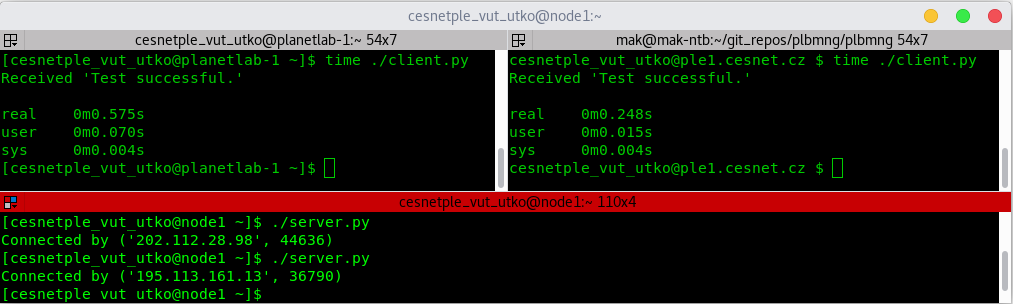
\includegraphics{obrazky/testingusecase}}
	\caption{Terminal view illustrating usage of PlanetLab Server Manager to find proper servers and run server/client echo script on them to measure round times of packets between Europe, China and America.}
	\label{fig:testingusecase}
\end{figure}

Script was copied into servers using Midnight Commander which provides extensive interface for managing files on both local and remote locations and can be seen in Figure~\ref{fig:midnightcommander}. As you can see by the results, the packets were successfully delivered and the packet round time were 0.248 seconds for Europe and 0.575 second for the China. This use case demonstrate very simple project but the same use case can be applied basically to any project as long as it use existing tools available on the servers. Even though only a bit above \SI{10}{\percent} servers are available, PlanetLab still offers a vast network of nodes for project testing.

\begin{figure}[H]
	\centering
	\scalebox{0.55}{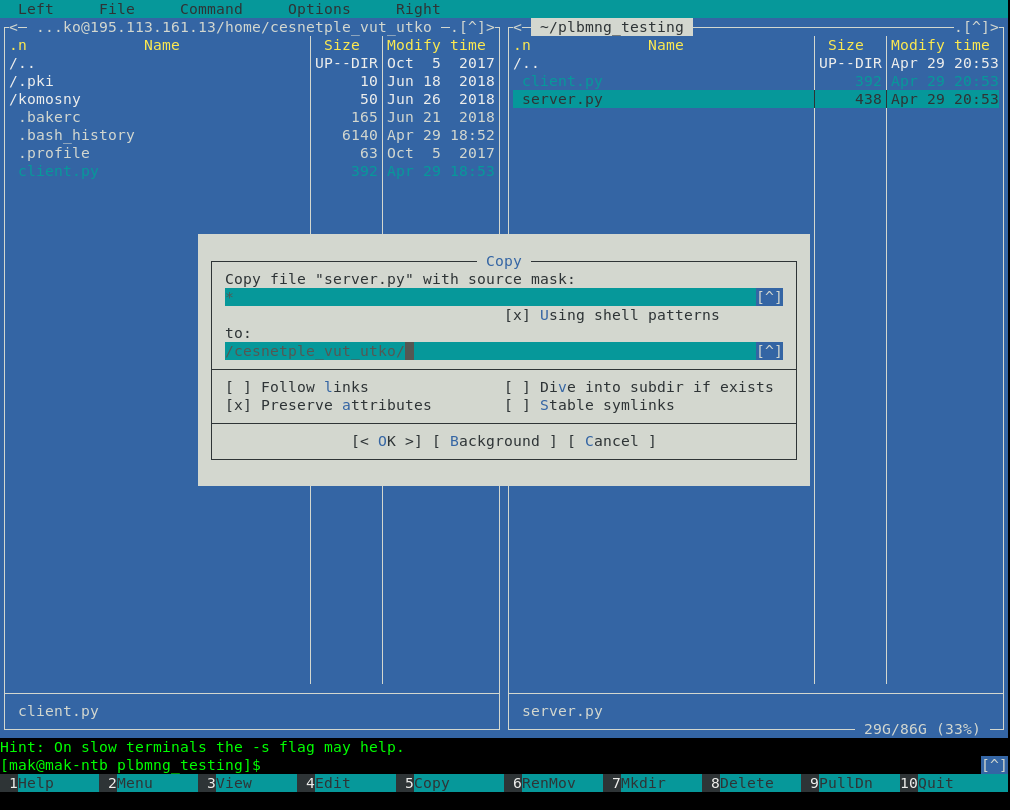
\includegraphics{obrazky/midnightcommander}}
	\caption{Illustration of midnight commander used to copy scripts from localhost (green rectangle) to a remote server (red rectangle) inside the PlanetLab network.}
	\label{fig:midnightcommander}
\end{figure}

{\noindent\begin{minipage}{\linewidth}
		\begin{lstlisting}[language=Python, numbers=left, label={lst:echoserver}, caption=Code of echo server., frame=single, showstringspaces=false, keywordstyle=\color{blue},captionpos=b]
#!/usr/bin/python

#Demo echo server for use case example
import socket

SOURCE_HOST = source_server_ip
PORT = 8765

s = socket.socket(socket.AF_INET, socket.SOCK_STREAM)
s.bind((SOURCE_HOST, PORT))
s.listen(1)
conn, addr = s.accept()
print 'Connected by: ', addr
while 1:
	data = conn.recv(1024)
	if not data:
		break
	conn.send(data)
	conn.close()
		\end{lstlisting}
	\end{minipage}

{\noindent\begin{minipage}{\linewidth}
		\begin{lstlisting}[language=Python, numbers=left, label={lst:echoclient}, caption=Code of echo client., frame=single, showstringspaces=false, keywordstyle=\color{blue},captionpos=b]
#!/usr/bin/python

#Demo echo client for use case example
import socket

TARGET_HOST = target_server_ip
PORT = 8765

s = socket.socket(socket.AF_INET, socket.SOCK_STREAM)
s.connect((TARGET_HOST, PORT))
s.send('Test successful.')
data = s.recv(1024)
s.close()
print 'Received: ', repr(data)
		\end{lstlisting}
\end{minipage}